
\begin{figure*}
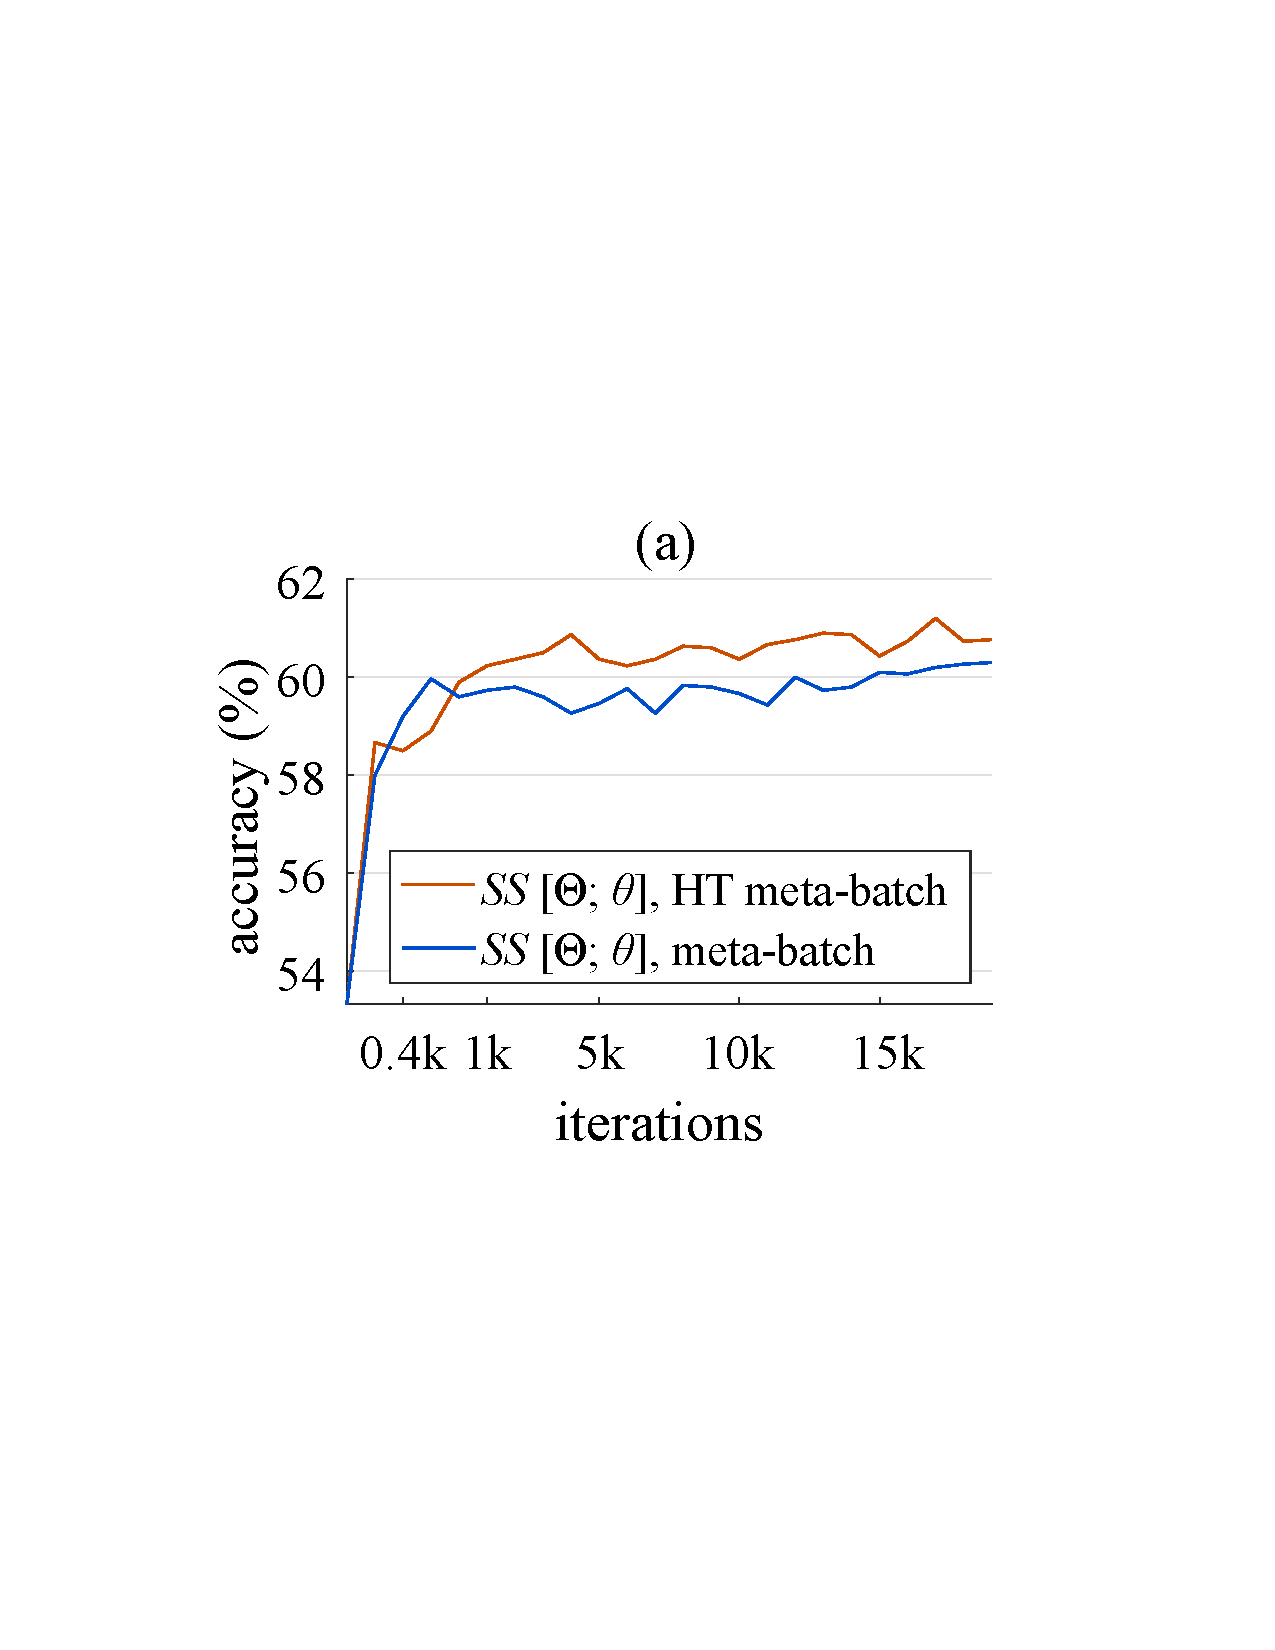
\includegraphics[height=1.09in]{mini1shot.pdf}
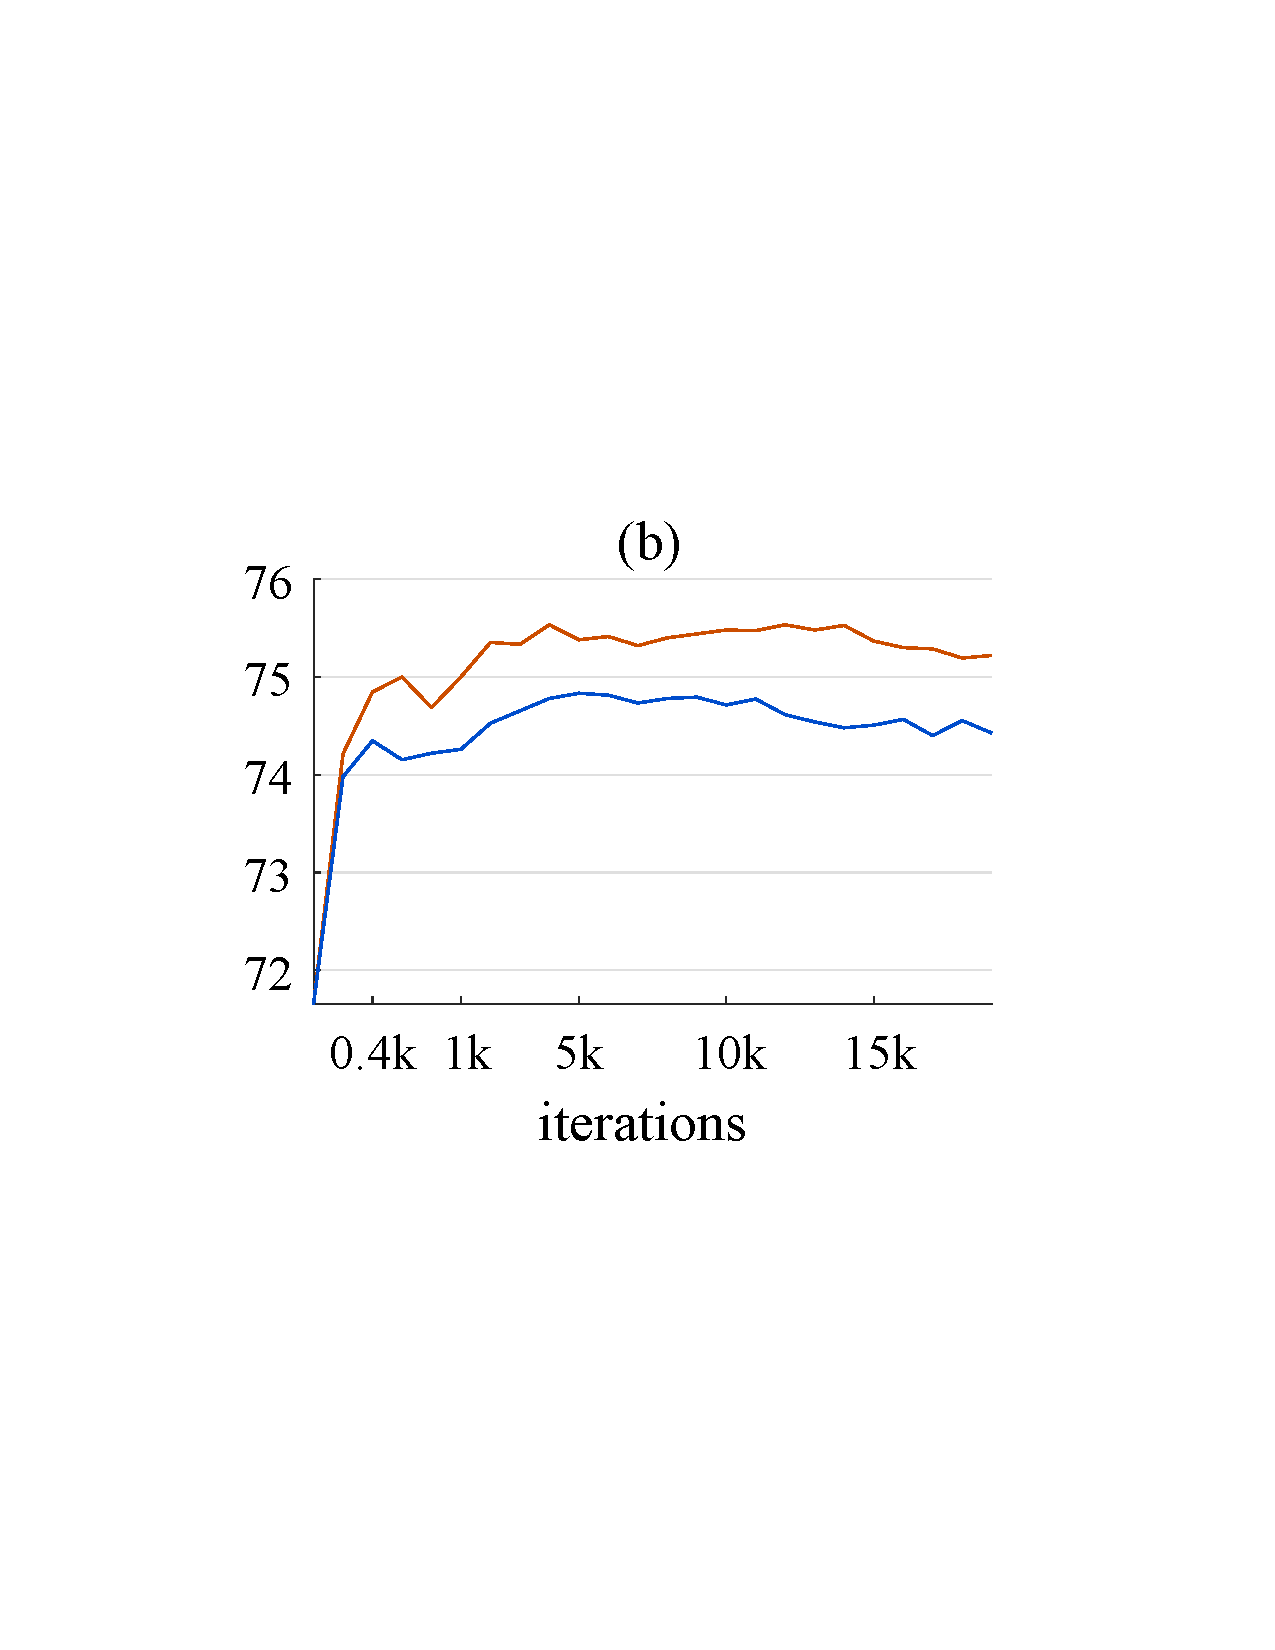
\includegraphics[height=1.09in]{mini5shot.pdf}
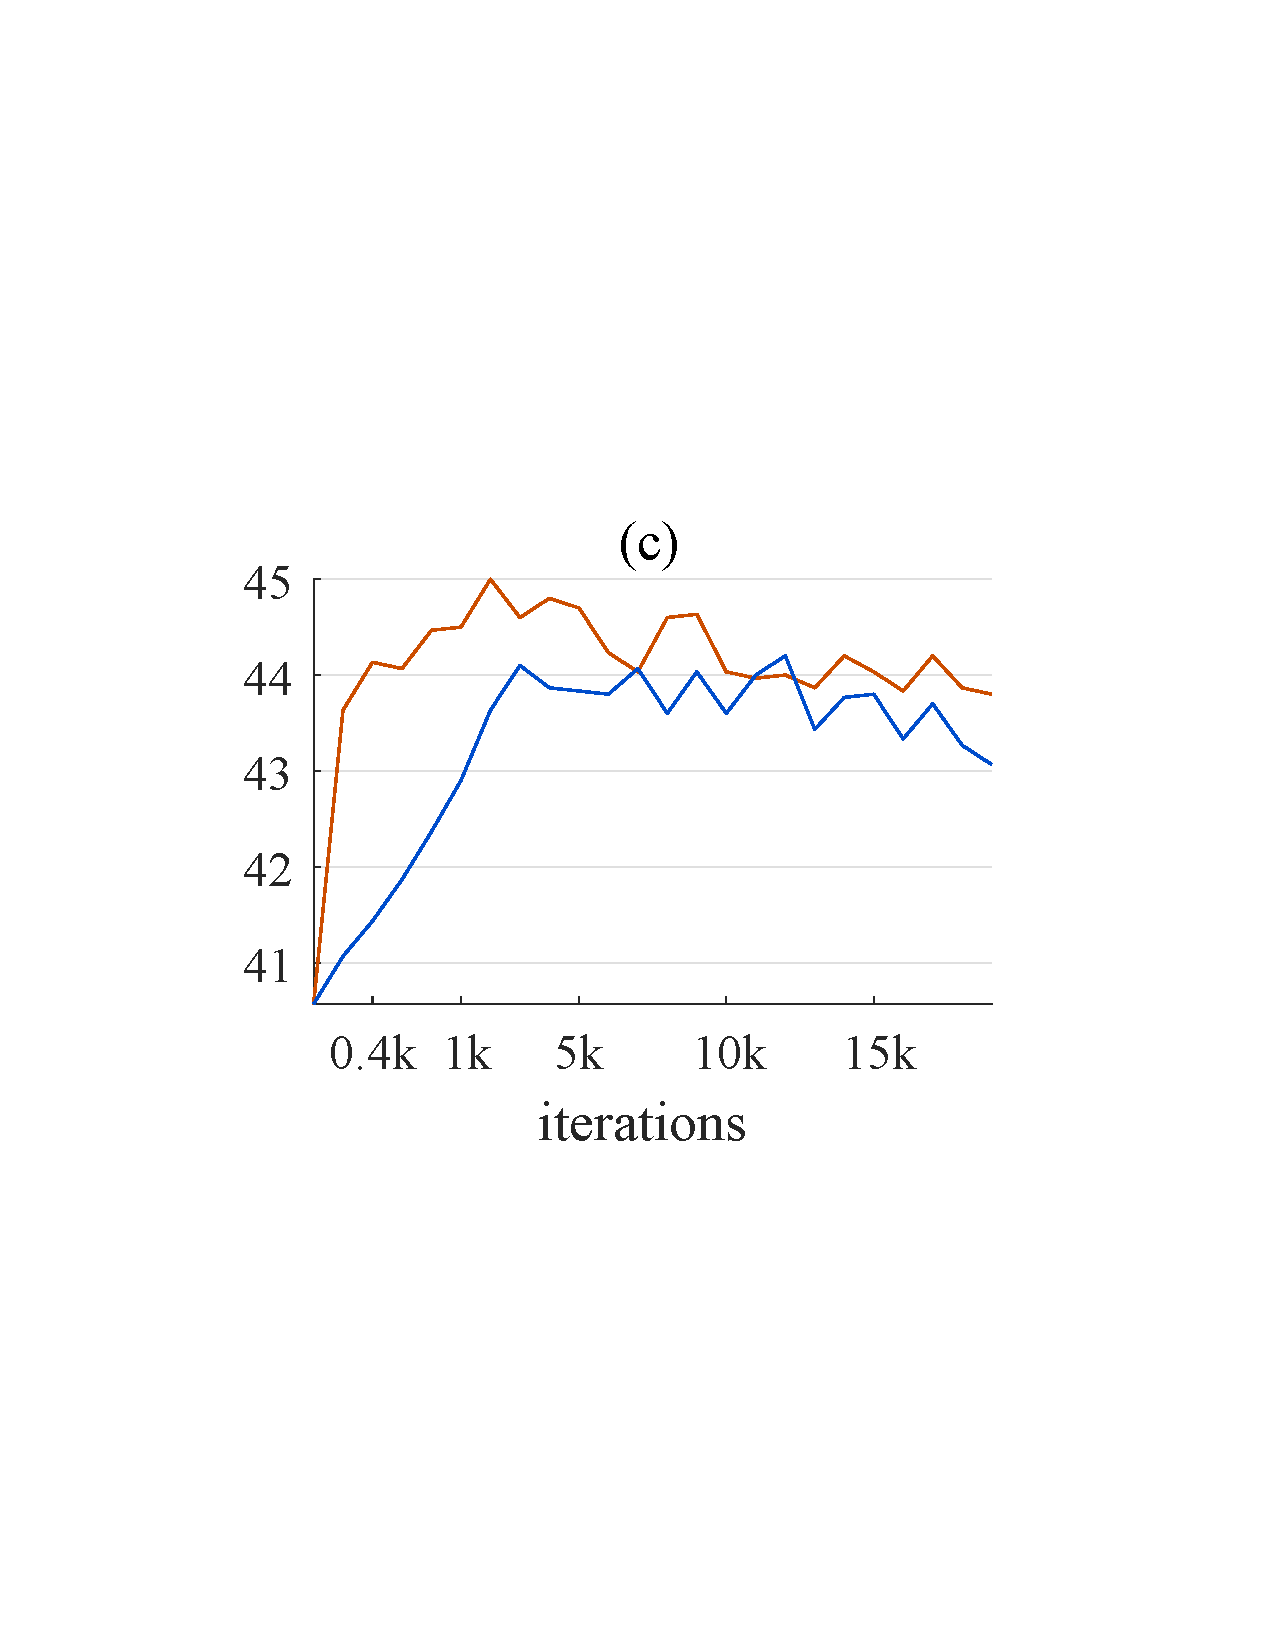
\includegraphics[height=1.09in]{fc1shot.pdf}
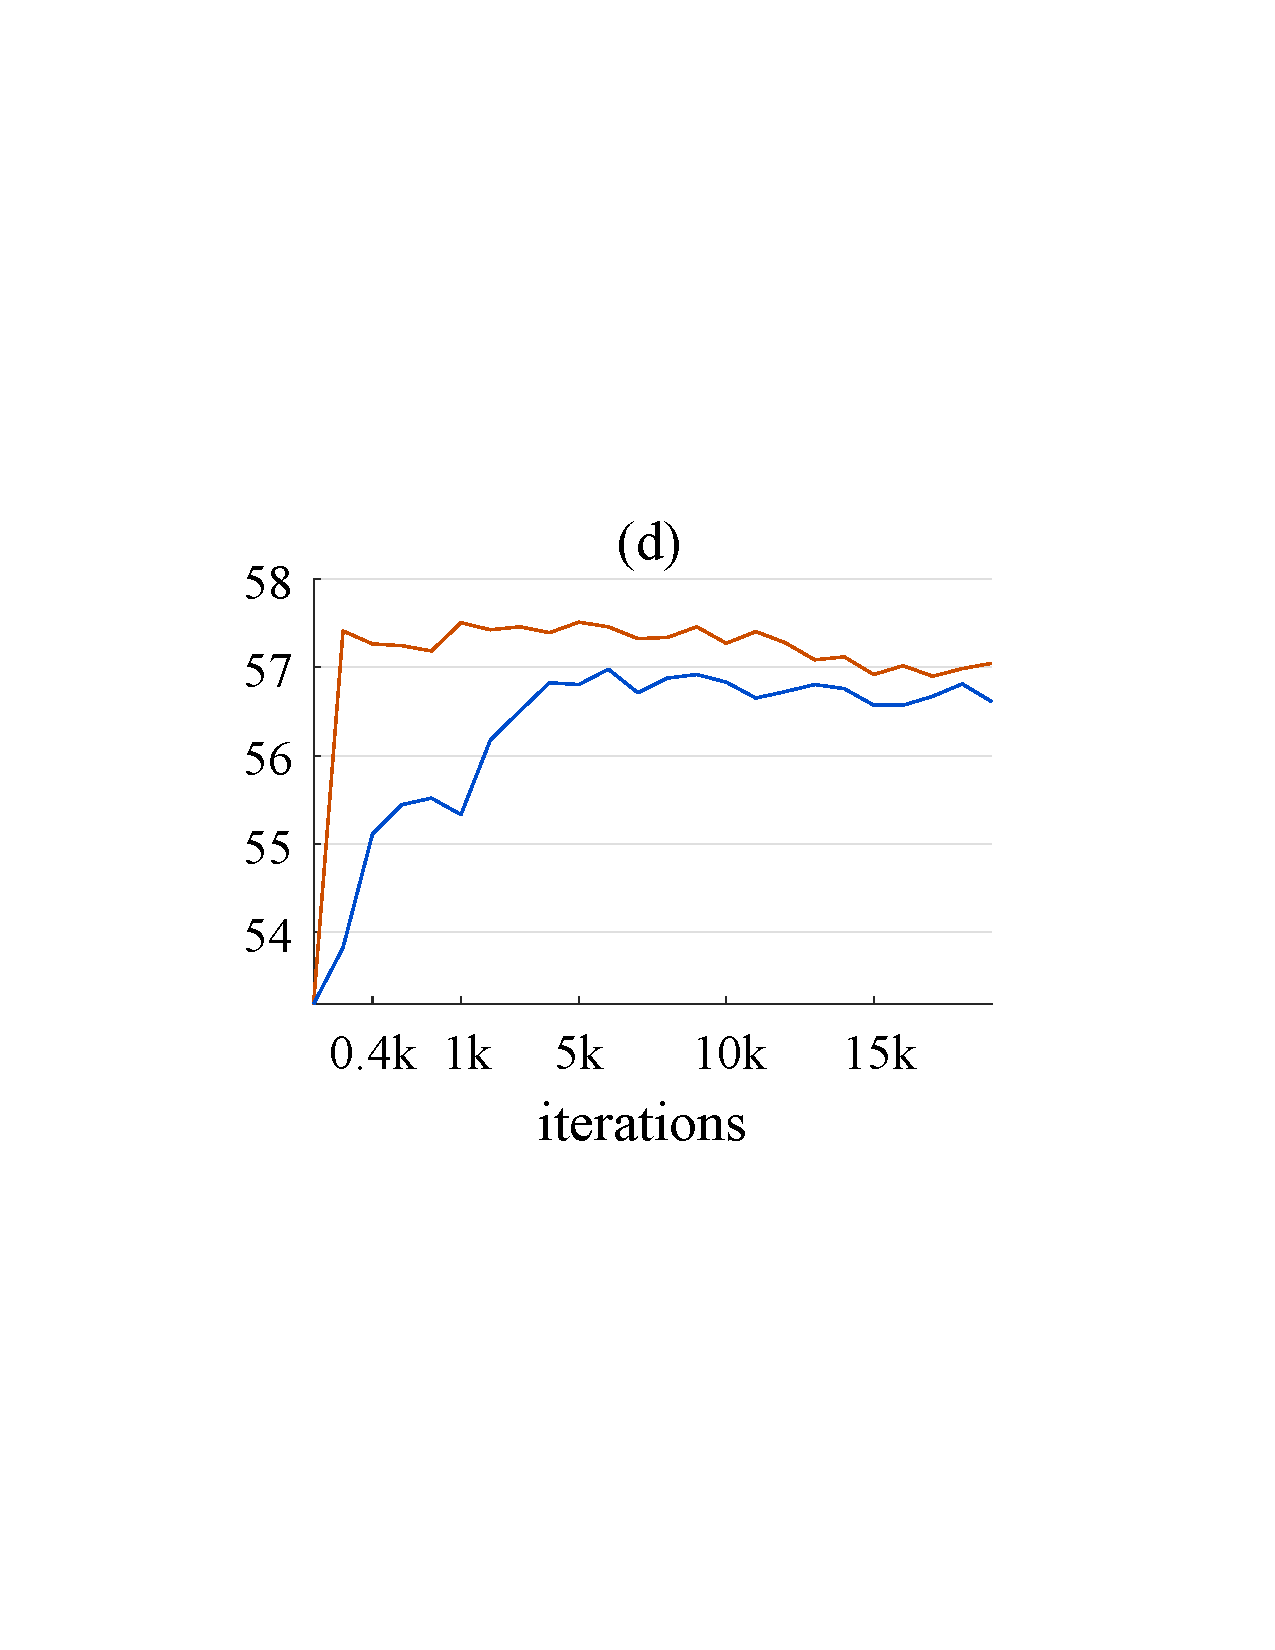
\includegraphics[height=1.09in]{fc5shot.pdf}
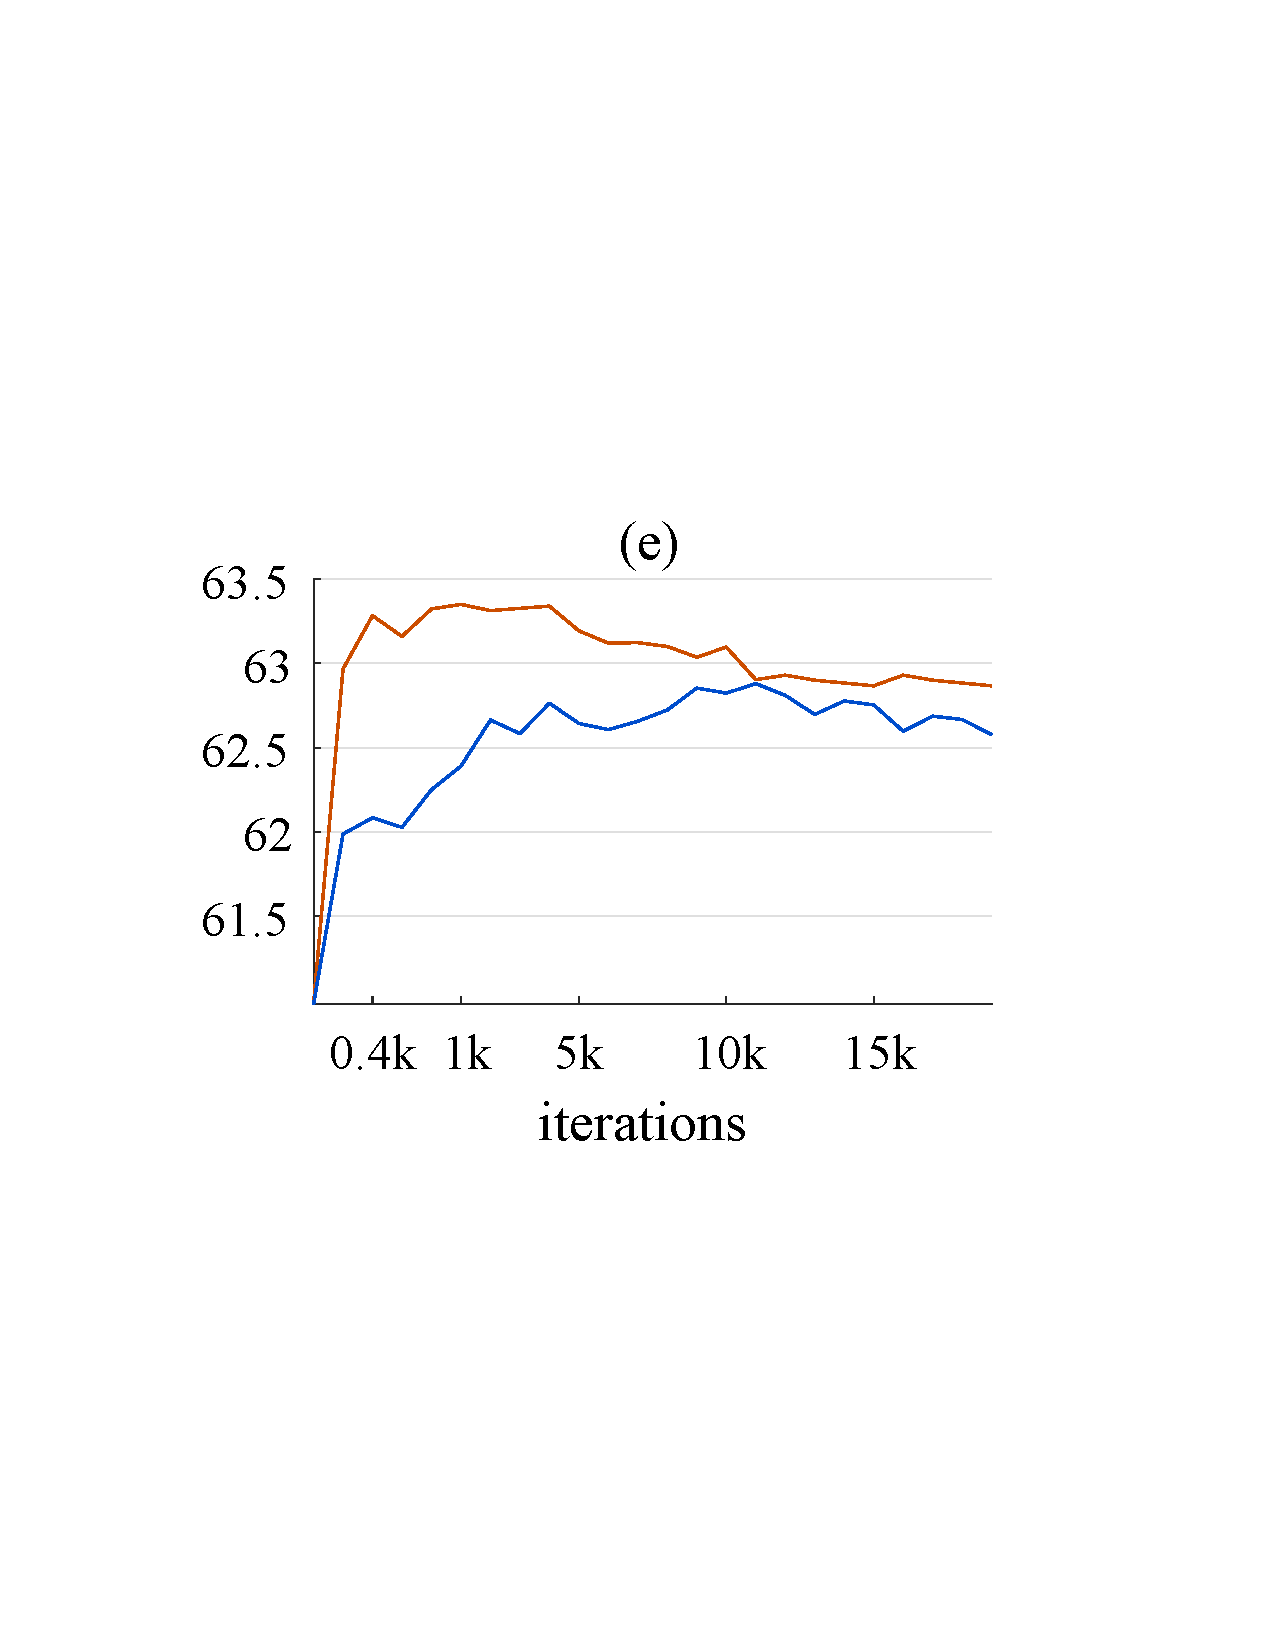
\includegraphics[height=1.09in]{fc10shot.pdf}
\caption{(a)(b) show the results of 1-shot and 5-shot on miniImageNet; (c)(d)(e) show the results of 1-shot, 5-shot and 10-shot on FC100.}
\vspace{-0.3cm}
\label{fig_mini_fc100}
\end{figure*}

\subsection{Ablation study setting}
\label{sec_setting}

In order to show the effectiveness of our approach, we design some ablative settings: 
%
two baselines without meta-learning but more classic learning,
three baselines of \emph{Fine-Tuning} (\emph{FT}) on smaller number of parameters (Table~\ref{tab_ablation_study}), and
%
two MAML variants using our deeper pre-trained model and HT meta-batch (Table~\ref{table_mini} and Table~\ref{table_fc100}).
Note that the alternative meta-learning operation to \emph{SS} is the \emph{FT} used in MAML.
Some bullet names are explained as follows.

\myparagraph{\emph{update} $[\Theta; \theta]$ (or $\theta$).} 
There is no meta-training phase. During test phase, each task has its whole model $[\Theta; \theta]$ (or the classifier $\theta$) updated on $\mathcal{T}^{(tr)}$, and then tested on $\mathcal{T}^{(te)}$.

\myparagraph{\emph{FT} $[\Theta 4; \theta]$ (or $\theta$).}
These are straight-forward ways to define a smaller set of meta-learner parameters than MAML.
We can freeze low-level pre-trained layers and meta-learn the classifier layer $\theta$ with (or without) high-level CONV layer $\Theta 4$ that is the 4th residual block of ResNet-12.
